\section{What is one of your earliest childhood memories?}
It is hard to know what my earliest childhood memory is but I do remember sitting on a stool by the wash bowl in the kitchen and having my hair combed and then braided.
Combing hair was most often my mother's domain but I have a memory that on a Sunday morning when my mother was quite busy with the getting ready for church details.
My father would set me up on the stool and comb out any knots in my hair so that I was ready for my mother to swoop in and finish me up with the braiding.
We did not go away from home with hair not braided.
That could have been like leaving without being completely dressed.

\begin{figure}
\centering
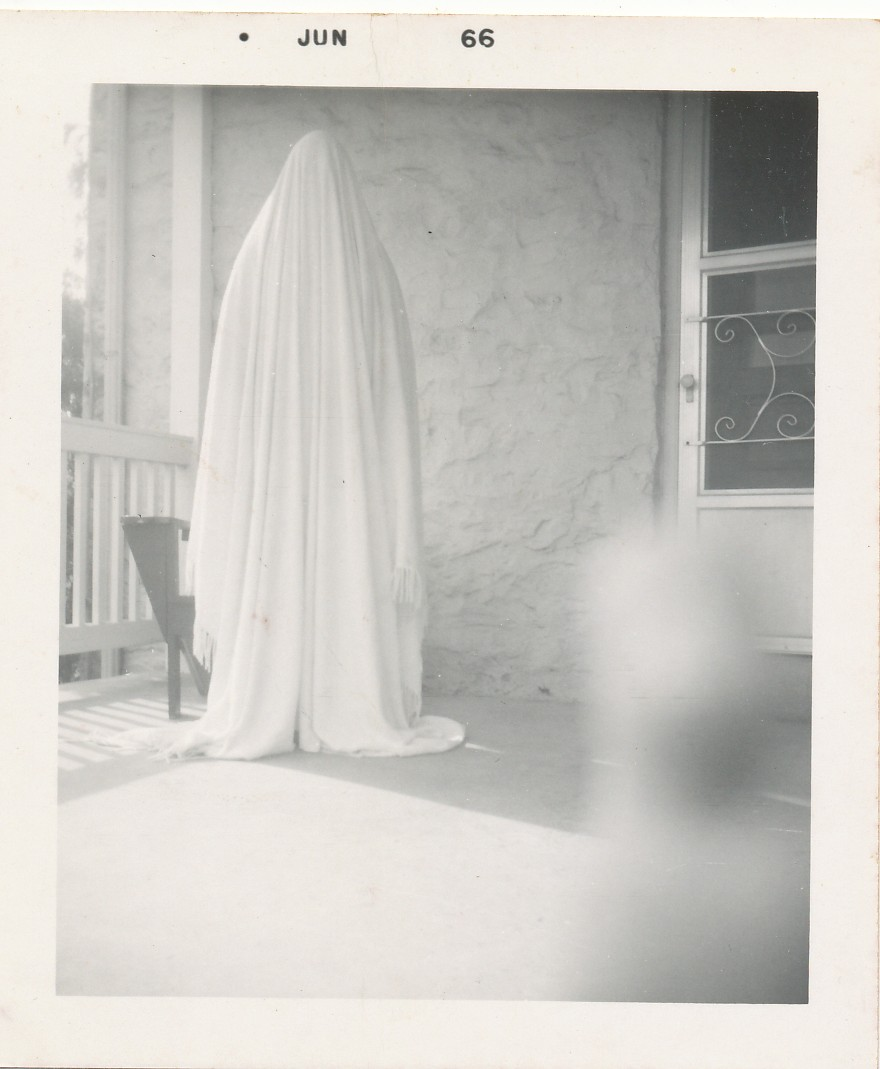
\includegraphics[width=0.6\textwidth]{childhood/1.jpg}
\caption{
The picture posted here was more likely taken on a Saturday afternoon when the 3 Aunties were making their weekly visit.
I had likely had my hair washed and I was waiting for it to dry.
I believe that this picture came from one of the Aunt's cameras.
}
\end{figure}

\begin{figure}
\centering
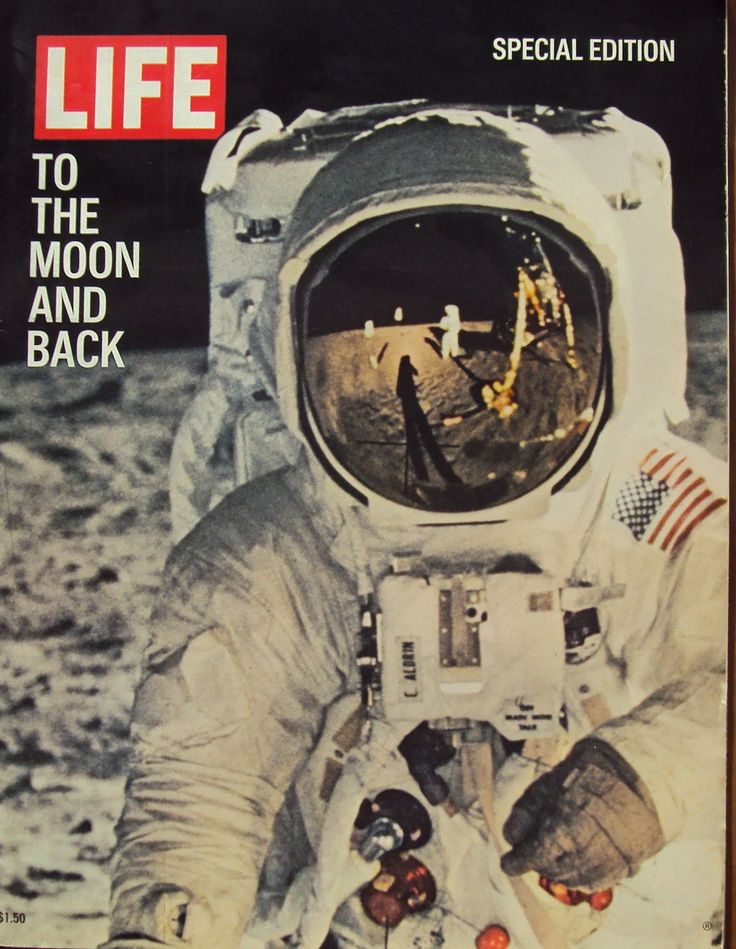
\includegraphics[width=0.6\textwidth]{childhood/2.jpg}
\caption{
Here I am holding my baby sister Rachel who was born 2 years after me in November 1954.
So here I am having just turned 2 years old.
}
\end{figure}
\begin{figure}
\centering
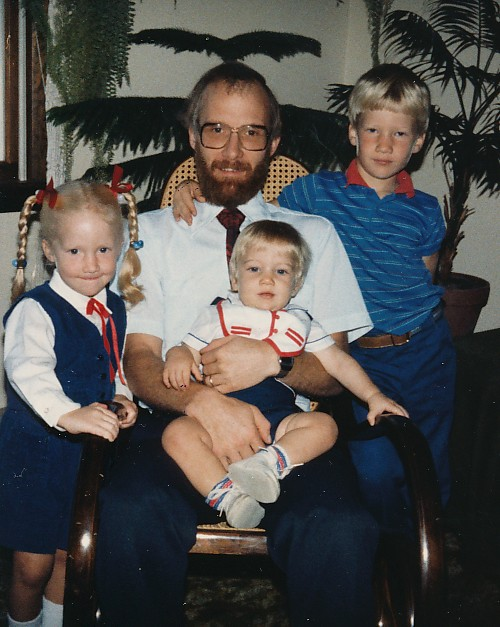
\includegraphics[width=1.0\textwidth]{childhood/3.jpg}
\caption{
Here you can see that Mary and I have two braids.
Rachel's hair is not long enough for braids.
I expect our ages are Mary 5, me 4 and Rachel 2 years.
}
\end{figure}
